\chapter{Tensor formalism}
\section{Introduction to tensors}
As we anticipated earlier in our discussion any couple of IRFs $\irf{R}, \irf{R}'$ can be obtained by using two transformations:
\begin{enumerate}
  \item Rotation, in order to make the axis be aligned \label{rotation_transformation}
  \item Translation, in order to make the origins coincide at some point in time \label{shift_transformation}
\end{enumerate}
If we can apply both \eqref{rotation_transformation} and \eqref{shift_transformation} we are in the so called \textbf{Poincarè group}, instead, if we only apply \eqref{rotation_transformation} we are in the \textbf{Lorentz group}, which, of course is a subgroup of the Poincarè group.\\
We also said that any event in Special Relativity has 4 coordinates $(x,y,z,t)$, but the Lorentz matrix $\lm$ has a better form if we consider the coordinates $(ct,x,y,z)$, so let us define a general vector:
\begin{equation}
  \begin{pNiceMatrix}
    x^0 \\[8pt]
    x^1 \\[8pt]
    x^2 \\[8pt]
    x^3
  \end{pNiceMatrix} =
  \begin{pNiceMatrix}
    ct \\[8pt]
    x \\[8pt]
    y \\[8pt]
    z
  \end{pNiceMatrix}
\end{equation}
With this we can also define a new 4-dimensional space where every point represents an event:
\begin{definition}{$\mink$ Minkowski spacetime}
  Minkowski spacetime $\mink$ is a 4-dimensional vector space where a generic element is defined by the coordinates $(x^0, x^1, x^2, x^3)$
\end{definition}
If we look back at the Lorentz transformations and use theory from linear algebra we can see that a new coordinate can be expressed in the form:
\begin{equation}
  x'^{\mu} = \bigsum_{\nu = 0}^{3} \pdv{x'^{\mu}}{x^{\nu}} x^{\nu}
\end{equation}
So a Lorentz transformation is just a change of coordinates in $\mink$. We will adopt 3 main conventions in order to make notation easier to read:
\begin{enumerate}
  \item Latin indeces are only related to the spatial coordinates (ex. $j=1,2,3$)
  \item Greek indeces represent every coordinate (ex. $\nu=0,1,2,3$)
  \item \textbf{Einstein summation convention} states that any repeated index implies a summation $\brackets{\text{ex. } \bigsum_{\nu = 0}^{3} \pdv{x'^{\mu}}{x^{\nu}} x^{\nu} \rightarrow \pdv{x'^{\mu}}{x^{\nu}} x^{\nu}}$
\end{enumerate}
Looking at the transformation of coordinates it is easy to see that we can put any element that multiplies the old coordinate in a matrix and express a change of coordinate as a matrix multiplied by a vector. In particular the elements of this matrix will be the elements of $\lm$.\\
Now we are ready to introduce the concept of \textbf{tensors}:
\begin{definition}{Tensors}
  Tensors are objects that are invariant under a change of coordinates in $\mink$
\end{definition}
The components of a tensor might change, but not the tensor itself. This is not a new concept, since this is the behaviour of vectors in the usual Euclidean space:
\begin{figure}[H]
    \begin{minipage}{0.5\textwidth}
     \centering
     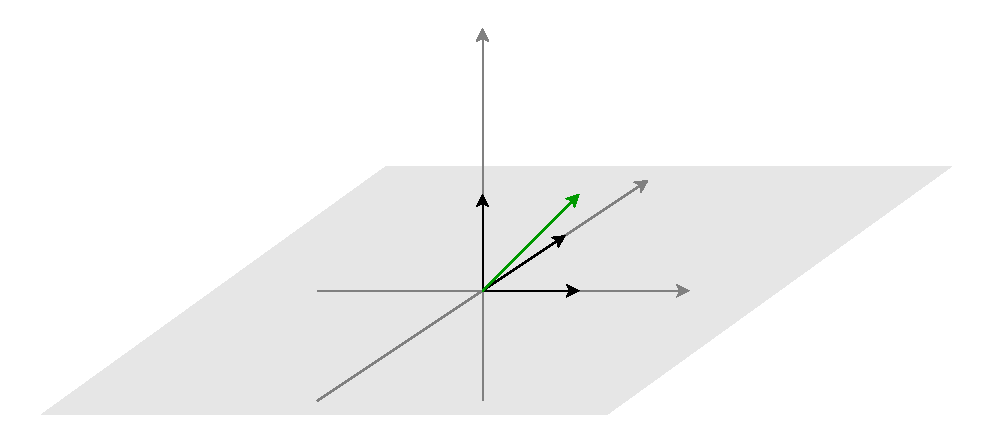
\includegraphics[width=1\linewidth]{res/svg/vector.drawio}
     \caption{Vector in $\mathcal{B}$}
   \end{minipage}\hfill
   \begin{minipage}{0.5\textwidth}
     \centering
     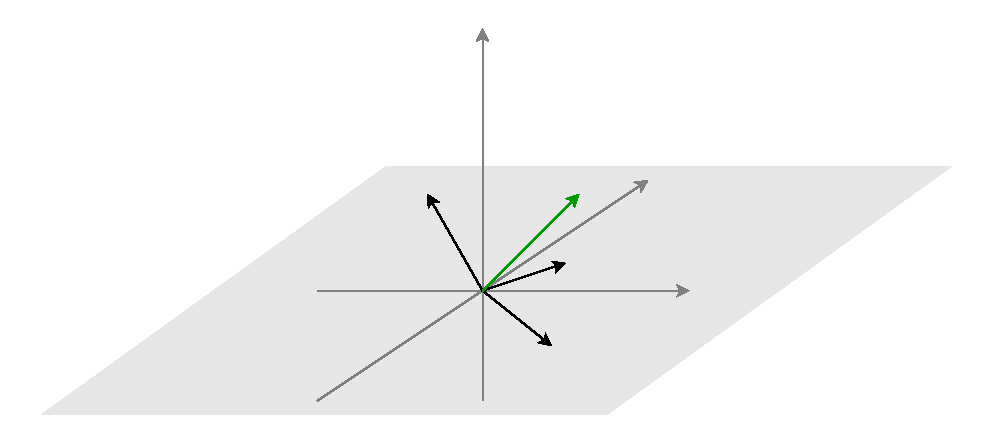
\includegraphics[width=1\linewidth]{res/svg/vettore_new.drawio}
     \caption{Vector in $\mathcal{B}'$}
   \end{minipage}
\end{figure}
Thus we want to write our equations using tensors in the form:
\begin{equation}
  \text{Tensor} = ( \,\dots\, )\;\text{Tensor}
\end{equation}
Lets now dive into more detail and see what types of tensors exist.
\subsection{Order 0 tensors: Scalar fields}
Scalar quantities are invariant under a change of coordinates, for example phase is a scalar field and thus it is invariant:
\begin{equation}
  \phi \longrightarrow \phi' = \phi
\end{equation}
\subsection{Order 1 tensors}
There are two types of order 1 tensors, the first ones are called \textbf{4-vectors}. But what are the prototypes of 4-vectors? As we said we want to obtain a new 4-vector by multipling it by something, in this case the Lorentz matrix $\lm$. If we simply take the vector:
\begin{equation}
  \begin{pNiceMatrix}
    x^0 \\[8pt]
    x^1 \\[8pt]
    x^2 \\[8pt]
    x^3
  \end{pNiceMatrix}
\end{equation}
as the base for our transformations we encounter a problem. If we make a transformation in the Poincarè group the transformations of the coordinates are no longer homogeneous, and so we cannot express the transformation as a simple matrix multiplication, instead we avoid this problem by using the differentials of the coordinates and so our prototype of a 4-vector will be:
\begin{equation}
  \begin{pNiceMatrix}
    \diff{x^0} \\[8pt]
    \diff{x^1} \\[8pt]
    \diff{x^2} \\[8pt]
    \diff{x^3}
  \end{pNiceMatrix}
\end{equation}
And so we will call a 4-vector anything that transforms like $\diff{x^{\mu}}$:
\begin{equation}
  \diff{x'^{\mu}} = \pdv{x'^{\mu}}{x^{\nu}} \diff{x^{\nu}}
\end{equation}
Recall that the elements $\pdv{x'^{\mu}}{x^{\nu}}$ are the elements of the Lorentz matrix and so they can be written as:
\begin{equation}
  \pdv{x'^{\mu}}{x^{\nu}} = \lm^{\mu}_{\nu}
\end{equation}
Leading to the transformations equations of a 4-vector in the desired form:
\begin{equation}
  \boxed{\diff{x'^{\mu}} = \lm^{\mu}_{\nu} \diff{x^{\nu}}}
\end{equation}
Finally we can say:
\begin{equation}
  \tensor{A}{^{\mu}} \text{ is a 4-vector } \iff A'^{\mu} = \lm^{\mu}_{\nu} \tensor{A}{^{\nu}}
\end{equation}
We also call those tensors \textbf{contravariant vectors}.\\
The second type of order 1 tensors are called covariant vectors or \textbf{covectors}. Let's take the four gradient of a scalar field:
\begin{equation}
  \pdv{\phi}{x'^{\mu}}
\end{equation}
By applying the chain rule we have:
\begin{equation}
  \pdv{\phi}{x'^{\mu}} = \pdv{\phi}{x^{\mu}}\pdv{x^{\mu}}{x'^{\mu}}
\end{equation}
But the elements $\pdv{x^{\mu}}{x'^{\mu}}$ are the elements of the inverse Lorentz matrix $\lm^{-1}$ and thus the transformation can be written as:
\begin{equation}
  \pdv{\phi}{x'^{\mu}} = \brackets{\lm^{-1}}^{\nu}_{\mu} \pdv{\phi}{x^{\mu}}
\end{equation}
\subsection{Higher order tensors}
For higher order tensors the transformation is generated by the same amount of matrices as the order, for example an order 2 tensor can transform as follows:
\begin{equation}
  \tensor{F}{^{\prime}^\mu^\nu} = \tensor{\lm}{^{\mu}_{\alpha}}\tensor{\lm}{^{\nu}_{\beta}}F^{\alpha\beta}
\end{equation}
And so, in general, any index trasnforms with its corresponding Lorentz matrix. The same is of course valid for lower indeces and so this generates different cases:
\begin{itemize}
  \item Contravariant tensor of order 2:
  \begin{equation}
    \tensor{F}{^{\prime}^\mu^\nu} = \tensor{\lm}{^{\mu}_{\alpha}}\tensor{\lm}{^{\nu}_{\beta}}F^{\alpha\beta}
  \end{equation}
  \item Covariant tensor of order 2:
  \begin{equation}
    \tensor{F}{^{\prime}_\mu_\nu} = \brackets{\lm_{\mu}^{-1}}^{\alpha}\brackets{\lm_{\mu}^{-1}}_{\nu}^{\beta}F_{\alpha\beta}
  \end{equation}
  \item Mixed tensor of order 2:
  \begin{equation}
    \tensor{F}{^{\prime}^{\mu}_{\nu}} = \tensor{\lm}{^{\mu}_{\alpha}}\brackets{\lm_{\mu}^{-1}}_{\nu}^{\beta}F^{\alpha}_{\beta}
  \end{equation}
\end{itemize}
An example of a mixed tensor is the unit tensor:
\begin{equation}
  \delta^{\mu}_{\nu} \defineeq \begin{cases}
    1 \quad \text{if $\mu = \nu$} \\[8pt]
    0 \quad \text{if $\mu \neq \nu$}
  \end{cases}
\end{equation}
Which has the property:
\begin{equation}
  \begin{split}
    \tensor{A}{^{\mu}} = \delta^{\mu}_{\nu} \tensor{A}{^{\nu}} \\[8pt]
    \tensor{A}{_{\nu}} = \delta^{\mu}_{\nu} \tensor{A}{_{\mu}}
  \end{split}
\end{equation}
The unit tensor can also be represented in matrix form as:
\begin{equation}
  \begin{pNiceMatrix}
    1 & 0 & 0 & 0 \\[8pt]
    0 & 1 & 0 & 0 \\[8pt]
    0 & 0 & 1 & 0 \\[8pt]
    0 & 0 & 0 & 1
  \end{pNiceMatrix}
\end{equation}
But what is the difference between a contravariant and a covariant vector? This is not a general rule, but we can think of those entities as follows:
\begin{itemize}
  \item $\tensor{A}{^{\mu}}$ has upper index $\implies$ row index \begin{equation}
    \begin{pNiceMatrix}
      \tensor{A}{^0} \\[8pt] \tensor{A}{^1} \\[8pt] \tensor{A}{^2} \\[8pt] \tensor{A}{^3}
    \end{pNiceMatrix}
  \end{equation}
  \item $\tensor{A}{_{\mu}}$ has lower index $\implies$ column index \begin{equation}
    \begin{pNiceMatrix}
      \tensor{A}{_0} & \tensor{A}{_1} & \tensor{A}{_2} & \tensor{A}{_3}
    \end{pNiceMatrix}
  \end{equation}
  \item $F_{\mu}^{\nu}$ has an upper index which represents a row and a lower index which represents a column
  \item $F_{\mu \nu}$ has both lower indeces and the first one is associated with a row while the second one with a column (this is valid also when both are upper indeces)
\end{itemize}
\section{Metric properties of spacetime}
In the Euclidean space $\mathbb{E}^3$ the distance between two points $A$ and $B$ is simply the 2-norm (also called Euclidean norm) of the vector. For an infinitesimal displacement $\diff{\vec{r}}$ we have:
\begin{equation}
  \begin{split}
    \diff{\vec{r}}^2 &= \diff{x}^2 + \diff{y}^2 + \diff{z}^2 = \diff{\vec{r}} \cdot \diff{\vec{r}} = \\[8pt]
    &= \diff{x}\diff{x} + \diff{y}\diff{y} + \diff{z}\diff{z} = \\[8pt]
    &= \begin{pNiceMatrix}
      \diff{x} & \diff{y} & \diff{z}\diff{z}
    \end{pNiceMatrix}
    \begin{pNiceMatrix}
      \diff{x} \\[8pt] \diff{y} \\[8pt] \diff{z}
    \end{pNiceMatrix} = \\[8pt]
    &= \begin{pNiceMatrix}
      \diff{x} & \diff{y} & \diff{z}
    \end{pNiceMatrix}
    \begin{pNiceMatrix}
      1 & 0 & 0 \\[8pt] 0 & 1 & 0 \\[8pt] 0 & 0 & 1
    \end{pNiceMatrix}
    \begin{pNiceMatrix}
      \diff{x} \\[8pt] \diff{y} \\[8pt] \diff{z}
    \end{pNiceMatrix}
  \end{split}
\end{equation}
So in the definition of distance in the Euclidean space we implicitly used the identity matrix in order to be able to multiply a row vector with a column vector. But there is no actual constrain that should limit us to use only the identity matrix, as a matter of fact this is just a particular case where the identity matrix is used as the \textbf{metric tensor}. In principle we could define infinitely many ways to calculating distance just by changing the metric tensor, but we are interested to what happens in $\mink$. We already defined the distance between two events ad the invariant quantity:
\begin{equation}
  \diff{s}^2 = c^2\diff{t}^2 - \diff{x}^2 - \diff{y}^2 - \diff{z}^2
\end{equation}
And so it is not surprising that the metric tensor in $\mink$ is:
\begin{equation}
  \tensor{g}{_\mu_\nu} \defineeq
  \begin{pNiceMatrix}
    1 & 0 & 0 & 0 \\[8pt]
    0 & -1 & 0 & 0 \\[8pt]
    0 & 0 & -1 & 0 \\[8pt]
    0 & 0 & 0 & -1
  \end{pNiceMatrix}
\end{equation}
And so the infinitesimal distance can also be written as:
\begin{equation}
  \diff{s}^2 =
  \begin{pNiceMatrix}
    \diff{x^0} & \diff{x^1} & \diff{x^2} & \diff{x^3}
  \end{pNiceMatrix}
  \begin{pNiceMatrix}
    1 & 0 & 0 & 0 \\[8pt]
    0 & -1 & 0 & 0 \\[8pt]
    0 & 0 & -1 & 0 \\[8pt]
    0 & 0 & 0 & -1
  \end{pNiceMatrix}
  \begin{pNiceMatrix}
    \diff{x^0} \\[8pt] \diff{x^1} \\[8pt] \diff{x^2} \\[8pt] \diff{x^3}
  \end{pNiceMatrix}
\end{equation}
Or, in tensor notation:
\begin{equation}
  \boxed{\diff{s}^2 = \diff{x}^{\mu} g_{\mu \nu} \diff{x}^{\nu}}
\end{equation}
The metric tensor is an order 2 covariant tensor, and it is invariant under Lorentz transformation:
\begin{equation}
  \tensor{g}{^{\prime}_\mu_\nu} = \tensor{\brackets{\lm^{-1}}}{^{\alpha}_{\mu}} \tensor{\brackets{\lm^{-1}}}{^{\beta}_{\nu}} \tensor{g}{_\alpha_\beta} = \tensor{g}{_\mu_\nu}
\end{equation}
This leads to what is called a \textbf{Pseudo-Riemannian geometry} which is different from Euclidean geometry.\\
From the definition of the metric tensor follows:
\begin{equation}
  \tensor{g}{^\mu^\nu} = \brackets{\tensor{g}{_\mu_\nu}}^{-1} = \tensor{g}{_\mu_\nu}
\end{equation}
So $\tensor{g}{^\mu^\nu} = \tensor{g}{_\mu_\nu}$ and the metric tensor is equal to its inverse. This connects covariant and contravariant tensors with the following relations:
\begin{equation}
  \begin{split}
    \tensor{A}{^{\mu}} = \tensor{g}{_\mu_\nu} \tensor{A}{^{\mu}} = (\,\dots) \tensor{A}{_{\nu}} \\[8pt]
    \tensor{A}{_{\mu}} = \tensor{g}{^\mu^\nu} \tensor{A}{_{\mu}} = (\,\dots) \tensor{A}{^{\nu}}
  \end{split}
\end{equation}
This operation is sometimes also called \textbf{index lowering} and the effect on the components is:
\begin{equation}
  \begin{pNiceMatrix}
    A^0 \\[8pt] A^1 \\[8pt] A^2 \\[8pt] A^3
  \end{pNiceMatrix}
  \longrightarrow
  \begin{pNiceMatrix}
    A_0 & -A_1 & -A_2 & -A_3
  \end{pNiceMatrix}
\end{equation}
So in general the metric tensor $\tensor{g}{_\mu_\nu}$ allows us to lower an index by switching sign to the spatial component $i = 1,2,3$. For example:
\begin{equation}
  \begin{split}
    &\partial_{\mu} \phi \quad \text{is a covector} \\[8pt]
    &\partial^{\mu} \phi \quad \text{is a contravariant vector}
  \end{split}
\end{equation}
And they are connected by the following relation:
\begin{equation}
  \begin{pNiceMatrix}
    \partial^0 \\[8pt] \partial^1 \\[8pt] \partial^2 \\[8pt] \partial^3
  \end{pNiceMatrix}
  \longrightarrow
  \begin{pNiceMatrix}
    \partial_0 & -\partial_1 & -\partial_2 & -\partial_3
  \end{pNiceMatrix}
\end{equation}
\subsection{Magnitude of a 4-vector}
We define the magnitude of a 4-vector in the same way as $\diff{x}^{\mu} \rightarrow \diff{s}^2 = \brackets{\diff{x^0}}^2 - \brackets{\diff{x^1}}^2 - \brackets{\diff{x^2}}^2 - \brackets{\diff{x^3}}^2$. And so we have:
\begin{equation}
  \diff{s}^2 = \diff{x}^{\mu} \tensor{g}{_\mu_\nu} \diff{x}^{\nu} = \diff{x}^{\mu} \diff{x}_{\nu}
\end{equation}
Thus, for a generic tensor:
\begin{equation}
  \boxed{A^2 = A^{\mu} A_{\mu}}
\end{equation}
In fact, if we expand term by term we get:
\begin{equation}
  \begin{split}
    A^2 &= A^{0} A_{0} + A^{1} A_{1} + A^{2} A_{2} + A^{3} A_{3} = \\[8pt]
    &= A^{0} A^{0} - A^{1} A^{1} - A^{2} A^{2} - A^{3} A^{3} = \\[8pt]
    &= \brackets{A^{0}}^2 - \brackets{A^{1}}^2 - \brackets{A^{2}}^2 - \brackets{A^{3}}^2
  \end{split}
\end{equation}
\subsection{Scalar product of a 4-vector}
As we did for the magnitude we can define the scalar product between two tensors as:
\begin{equation}
  x^{\mu} \tensor{g}{_\mu_\nu} q^{\nu} = x^{\mu} q_{\mu} = x^{0} q^{0} - x^{1} q^{1} - x^{2} q^{2} -x^{3} q^{3}
\end{equation}
The condition of orthogonality follows from the definition of the scalar product:
\begin{equation}
  x^{\mu} \text{ is orthogonal to } q^{\nu} \iff x^{\mu} q_{\mu} = 0
\end{equation}
\section{Other properties}
The partial derivative of a tensor with respect to the coordinates is not, in general, a tensor.
\begin{equation}
  A^{\mu} \longrightarrow \pdv{A^{\mu}}{x^{\nu}}
\end{equation}
But if it was a tensor it would transform as an order 2 tensor (2 indices) with the matrices $\lm$ and $\lm^{-1}$. Lets see what happens:
\begin{equation}
  \pdv{A'^{\mu}}{x'^{\nu}} = \pdv{\brackets{\tensor{\lm}{_{\alpha}^{\mu}} A^{\mu}}}{x'^{\nu}}
\end{equation}
Since $\tensor{\lm}{_{\alpha}^{\mu}}$ does not depend on the coordinates its partial derivative is zero:
\begin{equation}
  \pdv{A'^{\mu}}{x'^{\nu}} = \tensor{\lm}{^{\mu}_{\alpha}} \pdv{A^{\mu}}{x'^{\nu}} = \tensor{\lm}{^{\mu}_{\alpha}} \pdv{A^{\mu}}{x^{\beta}}\pdv{x^{\beta}}{x'^{\nu}}
\end{equation}
But $\pdv{x^{\beta}}{x'^{\nu}}$ are the elements of $\tensor{\brackets{\lm^{-1}}}{^{\beta}_{\nu}}$ so we finally get:
\begin{equation}
  \pdv{A'^{\mu}}{x'^{\nu}} = \tensor{\lm}{^{\mu}_{\alpha}} \tensor{\brackets{\lm^{-1}}}{^{\beta}_{\nu}} \pdv{A^{\mu}}{x^{\beta}}
\end{equation}
This is how a mixed tensor transforms, so for Lorentz transformations the derivative of a tensor is still a tensor.\\
Another property of 4-vectors in $\mink$ is that they have a time component and 3 space components, so the lowering of an index can be obtained by just switching sign to the space associated vector:
\begin{equation}
  A^{\mu} = \brackets{A^0, \vec{A}} \rightarrow A_{\mu} = \brackets{A^0, -\vec{A}}
\end{equation}
